\documentclass[10pt]{article}
\usepackage[margin=1in]{geometry}
\usepackage{graphicx}
\graphicspath{{images/}{./}}  % first check 'images/' then the current directory

\usepackage{titlesec}
\usepackage{amsmath,amssymb}
\usepackage{booktabs}
\usepackage{caption}
\usepackage[hidelinks]{hyperref}
\usepackage{enumitem}

\title{\bfseries byron: Another Key-Value Store}
\author{%
  Michael Almeida\\
  \small CS265 Spring 2023\\
  \texttt{mia330@g.harvard.edu}%
}
\date{} % no date

\begin{document}
\maketitle

\section{Design Description}

\subsection{Introduction}
byron is a high-performance, latch-free NoSQL key-value store implemented in Rust using a Log-Structured Merge Tree (LSM) architecture. The system is designed for write-intensive workloads by leveraging cache-conscious design and hardware-friendly storage layouts. Core supporting data structures include memtables, SSTables, Bloom filters, and fence pointers, while core algorithms handle tasks such as compaction, Bloom filter allocation, and on-disk storage formatting.

\subsection{Technical Description}
This section provides a detailed overview of byron’s design considerations and technical architecture.

\subsubsection*{(A) On-Disk Data Layout}
\begin{figure}[htbp]
  \centering
  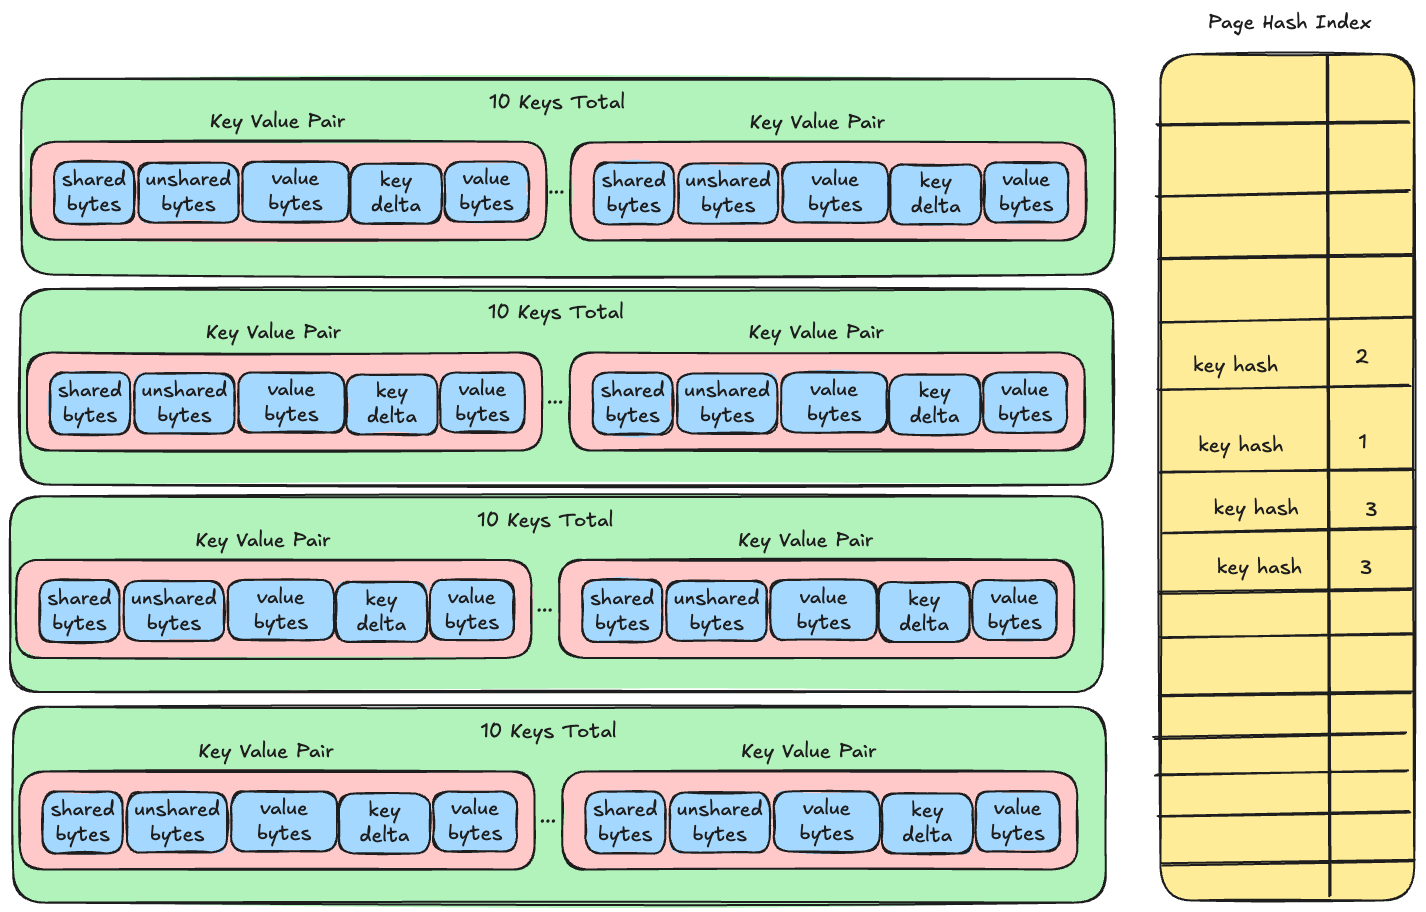
\includegraphics[width=0.8\textwidth]{sstable_full.png}
  \caption{SSTable on-disk layout.}\label{fig:SSTable}
\end{figure}

\paragraph{Goal}
Our overarching goal is to minimize disk I/O and CPU cache misses by optimizing the on-disk data layout.
byron uses a Log-Structured Merge Tree (LSM) architecture, and compacts stored data frequently to reduce fragmentation and improve read performance.
A key component of the LSM tree is the SSTable, which is an immutable on-disk file that stores sorted key-value pairs. The design of the SSTable is critical to achieving high performance in both read and write operations.
The SSTable is designed to be compact and efficient, with a focus on minimizing disk I/O and CPU cache misses.
In our design, we align SSTable blocks to 4 KB SSD pages for minimal random accesses and high sequential I/O throughput, and use key compression to pack more entries per page.

\paragraph{Design Elements}

\begin{description}[leftmargin=1em,labelwidth=*,itemsep=0.5ex]
  \item[Varint Encoding] (Integer metadata) (lengths, sequence numbers) are stored in a compact varint format to save bytes.
  \item[Delta Encoding (Prefix Compression)] Each key is recorded as the byte‐suffix that differs from its predecessor, greatly reducing size when keys share prefixes.
  \item[Restart Points] Every 10th key in a block is stored in full (not delta–encoded).  These “restart” keys bound the cost of an in‐block binary search.
  \item[Page Hash Index] An in‐memory array of each block’s first key lets you binary‐search the correct 4 KB page in $O(\log N)$ time, avoiding a full scan.
\end{description}

\paragraph{Rationale}
An SSTable is an immutable on‐disk file of sorted key–value pairs with the above optimizations.
Keys are serialized by first writing a varint length, then a byte‐slice delta from the previous key.
Within each 4 KB block, restart points ensure you never examine more than 9 other keys on average.
The restart‐pointer index (one key per block) lives in RAM, so most $\mathtt{GET}$s need at most one disk read—and none if the key isn’t present.

Together, prefix compression plus restart indexing typically save about 3 bytes per 32-byte key.
In skewed key distributions (e.g.\ sequential timestamps), the stored suffix length approaches a small constant, making delta encoding extremely efficient when keys share long prefixes.
Analysis in \S\ref{sec:SSTable Optimization Efficacy} elucidates the performance of these optimizations under expected bytes saved.

\paragraph{Variable Integer Width}
Instead of representing fields in our keys as flat integers, we instead use Variable-width Integers– a format popularized by the Protobufs project. Each byte in a varint consists of a continuation bit and a 7 bit payload– the continuation bit being there to let us know whether this bit is a continuation of the previous byte.
\begin{verbatim}
continuation bit | 0 1 2 3 4 5 6
\end{verbatim}

\paragraph{Delta Encoding}

\begin{figure}[htbp]
  \centering
  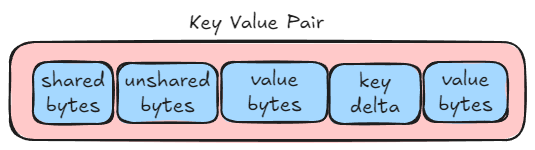
\includegraphics[width=0.8\textwidth]{key_value_pair.png}
  \caption{Key Value pair structure.}\label{fig:Key Value Pair}
\end{figure}

\begin{itemize}[itemsep=0pt, parsep=0pt]
  \item \texttt{shared\_bytes}: Shared prefix length with predecessor key.
  \item \texttt{unshared\_bytes}: Length of key suffix.
  \item \texttt{value\_bytes}: Length of the associated value.
  \item \texttt{key\_delta}: Remaining suffix of the key.
  \item \texttt{value}: Actual stored value.
\end{itemize}

Delta encoding is a technique used to compress data by storing only the differences between consecutive values. In the context of key-value pairs, this means that instead of storing the entire key, we only store the part of the key that differs from the previous key. This is particularly effective when keys are similar or share common prefixes.
For example, if we have two keys `key1` and `key2`, instead of storing both keys in full, we can store the length of the shared prefix (in this case, `key`) and then only store the differing part `1` and `2`. This reduces the amount of data that needs to be stored and can lead to significant space savings, especially when dealing with large datasets with many similar keys.

\paragraph{Restart Points and Page Hash Index}
\begin{figure}[htbp]
  \centering
  \begin{minipage}{0.48\textwidth}
    \centering
    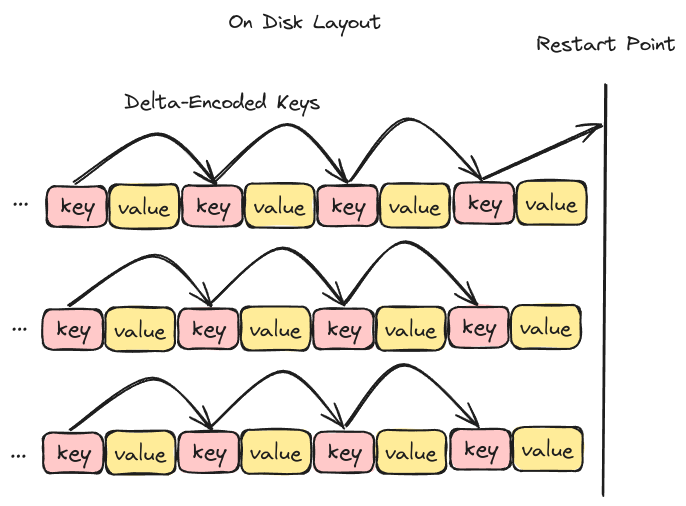
\includegraphics[width=\textwidth]{restart_points.png}
    \caption{Restart Points.}\label{fig:Restart Points}
  \end{minipage}
  \hfill
  \begin{minipage}{0.48\textwidth}
    \centering
    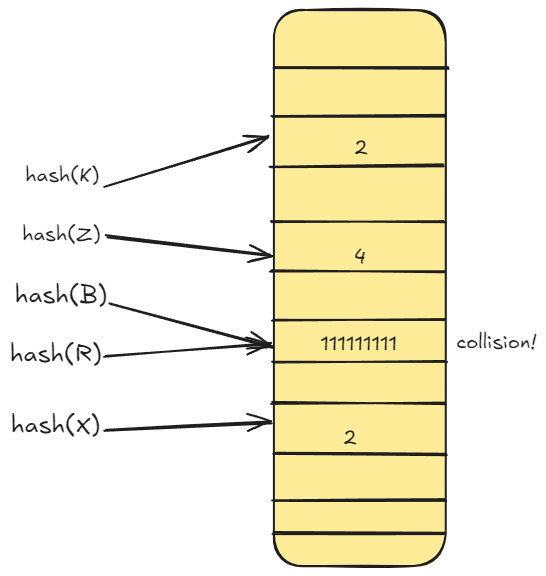
\includegraphics[width=\textwidth, height=0.33\textheight]{page_hash_index.png}
    \caption{Page Hash Index.}\label{fig:Page Hash Index}
  \end{minipage}
\end{figure}

The draw back to using Delta Encoding is that in order to find a key, we must then linear search the entire block. This is undesirable, as now we incur a cost of O(n), where n is the block size.
To combat this, we embed `Restart Points` in each block; and we do so at every 10th key.


\paragraph{Page Hash Index}

On their own, Restart points are saved as pointers at the end of a SStable in the footer. In order to beat Binary Searching these restart pointers, we need to do something else. This comes in the form of a Page Hash index.
Simply put, a page hash index matches a keys hash with it's restart point. Each entry has a maximum of 8 bits width, and points to a restart page. Implicitly, this means we can identify at most 256 restarts.
The amount of slots is the number of keys. This is a very simple hash table, so collisions are possible. In the case of there being a collision, we cancel the slot and default to binary search.

\paragraph{SSTable Footer}
In the common literature, footer of an SSTable contains metadata about the table, including the size of the table, the number of keys, and the location of the restart points. This information is used to quickly locate and access the data in the SSTable. The footer is also compressed to save space.
However, in byron, for simplicities sake, we store the page hash index and restart points in RAM.



\subsubsection*{(B) Memtable Data Structure Design}
\paragraph{Original and Enhanced Approach}
\begin{figure}[htbp]
  \centering
  \begin{minipage}{0.48\textwidth}
    \centering
    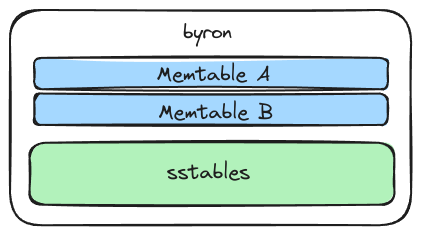
\includegraphics[width=\textwidth]{memtables.png}
    \caption{Double Buffered.}\label{fig:Double Buffered}
  \end{minipage}
  \hfill
  \begin{minipage}{0.48\textwidth}
    \centering
    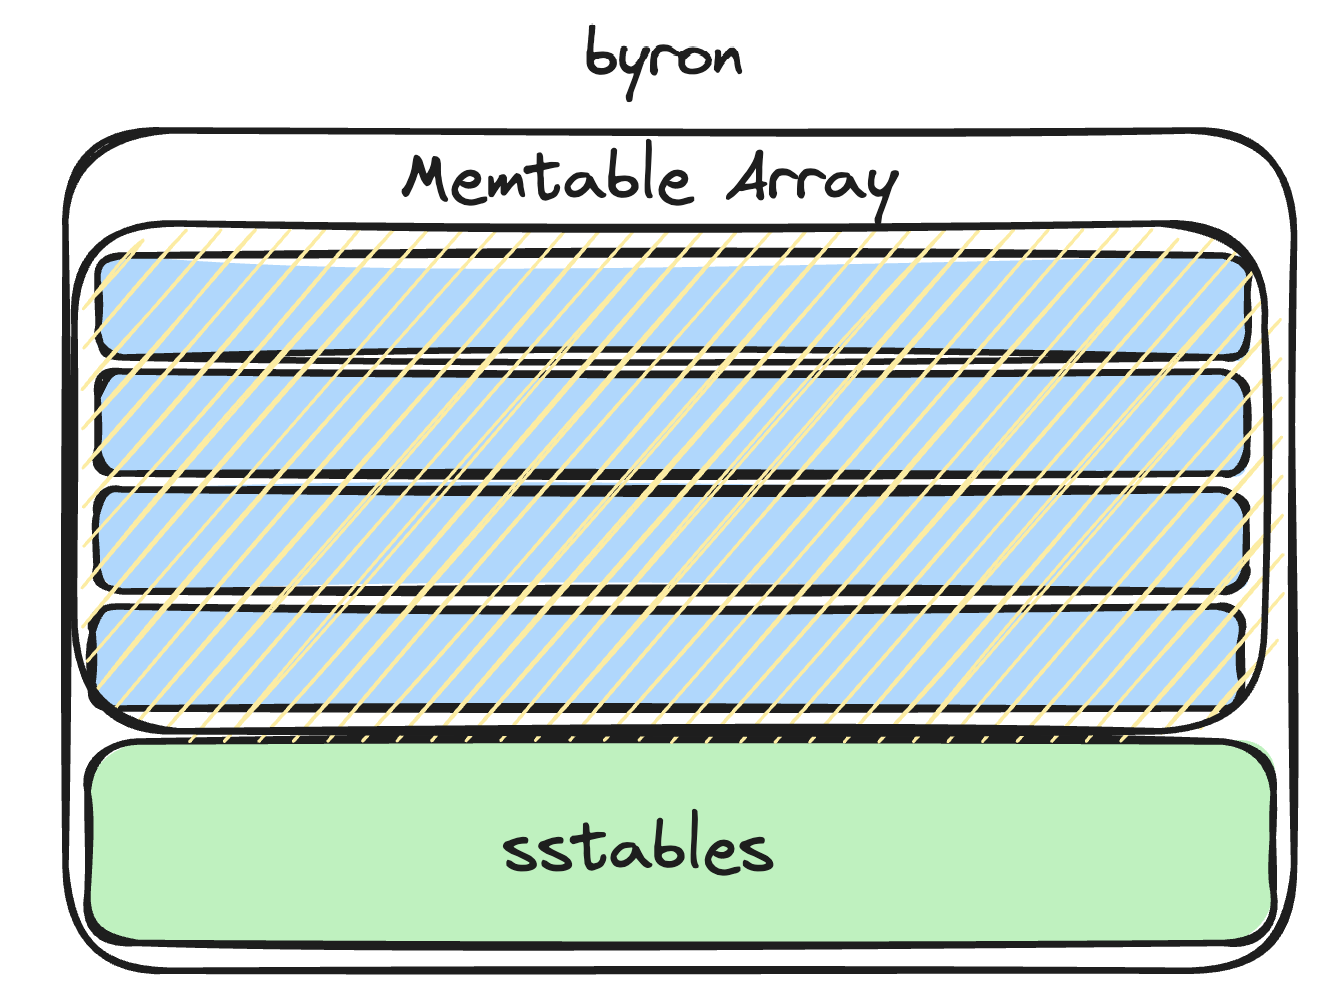
\includegraphics[width=\textwidth, height=0.33\textheight]{memtable_array.png}
    \caption{Skiplist array.}\label{fig:Skiplist array}
  \end{minipage}
\end{figure}


\paragraph{Goal}
The memtable serves as a fast, in-memory structure for buffering writes before they are flushed to disk. byron’s memtable is implemented as a lock-free skiplist, which provides efficient insertion and lookup while maintaining key order. This design ensures high performance for both writes and reads in a concurrent environment.

Originally, byron used a double-buffered vector for the memtable. While simple, this approach had limitations in terms of concurrency and performance. The skiplist implementation addresses these issues by offering better cache locality, reduced contention between threads, and thread-safe operations. Additionally, the skiplist is sourced from the battle-tested `crossbeam` library, which is optimized for performance and safety, allowing us to focus on higher-level optimizations.

Although the skiplist achieves $O(\log n)$ writes instead of the amortized $O(1)$ writes of the vector, it significantly improves over the vector’s $O(n)$ worst-case performance. Furthermore, the skiplist supports concurrent writes and reads, enabling multiple threads to operate simultaneously without blocking. This lock-free design leads to better overall throughput, making it well-suited for a high-performance key-value store.

\paragraph{Original Approach: Double-Buffered Vector}
\begin{description}[leftmargin=1em,labelwidth=*,itemsep=0.25ex]
  \item[Double buffers] Two memtables—“active” and “immutable”—hold writes. Once the active buffer reaches 2 MB, it becomes immutable and flushes in the background while new writes go into the other buffer.
  \item[Lock-free writes] Appends to the active vector are amortized $O(1)$ and require no locks for producers.
  \item[Linear scans for reads] GETs search both buffers linearly; for typical memtable sizes, this overhead remains low.
\end{description}

\paragraph{Enhanced Approach: Lock-Free Skiplist}
\begin{description}[leftmargin=1em,labelwidth=*,itemsep=0.5ex]
  \item[Crossbeam \texttt{SkipMap}] Replaced backing vectors with a lock-free skiplist offering thread-safe $O(\log n)$ inserts and lookups.
  \item[Memtable Array] Each memtable is a skiplist, and we maintain an array of memtables to allow for concurrent writes and reads. This allows us to have multiple active memtables, which can be flushed in parallel. Writes always hit memtable[0]
  \item[Built-in ordering] Eliminates the extra sort/merge step on flush—entries stream out in sorted order.
  \item[Improved cache locality] Skiplist nodes and allocators reduce cache-line bouncing; measured cache misses dropped from 10.69\% (vector) to 4.99\% (skiplist).
\end{description}

\paragraph{Flush Interface}
An inherent iterator on the skiplist streams sorted key–value pairs directly to a new SSTable file, enabling efficient sequential writes without additional merging.
The iterator is designed to be lock-free, allowing multiple threads to read from the skiplist while it is being modified. This ensures that the flush process does not block other operations, maintaining high throughput for concurrent writes.
There were a lot of challenges in parralellizing the flush process for the vector backed memtables-- however, flushing the skiplists was a lot easier and, in practice, the memtable array never gets larger than 2 memtables.

\paragraph{Vector Backed}
\begin{itemize}[leftmargin=1em,itemsep=0.25ex,parsep=0ex]
  \item \textbf{Time Complexity:}
  \begin{itemize}[leftmargin=1em,itemsep=0.25ex,parsep=0ex]
    \item Sorting and deduplication using a \texttt{BTreeMap} is $O(n \log n)$, where $n$ is the number of key-value pairs.
    \item Iterating through the \texttt{BTreeMap} is $O(n)$.
    \item Total flush complexity: $O(n \log n)$.
  \end{itemize}
  \item \textbf{Space Complexity:}
  \begin{itemize}[leftmargin=1em,itemsep=0.25ex,parsep=0ex]
    \item Two buffers: $O(n)$.
    \item Temporary \texttt{BTreeMap}: $O(n)$.
    \item Total: $O(n)$.
  \end{itemize}
  \item \textbf{Expected Runtime:}
  \begin{itemize}[leftmargin=1em,itemsep=0.25ex,parsep=0ex]
    \item Runtime is primarily dominated by sorting, which, under our previous assumptions for the structure of keys, means that they will be very small and rather quick.
    \item Disk flush operations themselves are asynchronous and minimize the impact on the main application performance.
  \end{itemize}
\end{itemize}

\paragraph{crossbeam-backed Memtable}
\begin{itemize}[leftmargin=1em,itemsep=0.25ex,parsep=0ex]
  \item \textbf{Time Complexity:}
  \begin{itemize}[leftmargin=1em,itemsep=0.25ex,parsep=0ex]
    \item \textbf{Writes/Reads:} Each \texttt{insert} or \texttt{get} is $O(\log n)$ in the skiplist.
    \item \textbf{Flush:} Streaming entries in sorted order is $O(n)$ with no extra sorting.
  \end{itemize}
  \item \textbf{Space Complexity:}
  \begin{itemize}
    \item N buffers: $O(n)$. (Usually this is 2, but we can have more if we want to.)
    \item Each skiplist node: $O(1)$.
    \item Total: $O(n)$.
  \end{itemize}
  \item \textbf{Expected Runtime:}
  \begin{itemize}[leftmargin=1em,itemsep=0.25ex,parsep=0ex]
    \item Runtime is primarily dominated by the skiplist operations, which are $O(\log n)$.
    \item Disk flush operations themselves are asynchronous and minimize the impact on the main application performance.
  \end{itemize}
\end{itemize}

\subsubsection*{(C) Bloom Filters \& Fence Pointers in Memory}

\paragraph{Goal}
The goal of the Bloom filter and fence pointer design is to minimize disk reads and enhance read performance. byron uses Bloom filters to probabilistically test key membership, skipping unnecessary SSTable reads, and fence pointers to index the first key of each block for efficient lookups. Together, they reduce disk I/O, improve cache efficiency, and accelerate read-heavy workloads by leveraging small, cache-friendly data structures.

\begin{description}[leftmargin=1em,labelwidth=*,itemsep=0.5ex]
  \item[Per‐SSTable Filters] Each SSTable has an in‐memory Bloom filter. On a \texttt{GET}, we query the filter first—if it says “not present,” we skip that SSTable entirely (no disk I/O).
  \item[Monkey‐Inspired Allocation] We distribute Bloom‐filter bits across LSM levels proportional to data volume, giving larger lower‐level tables more bits per key.
  \item[Performance Impact] Tuning the total filter budget from 100 K bits to 10 M bits per SSTable improved \texttt{GET} throughput by ~10\%, with diminishing returns beyond ~1 M bits.
  \item[Sparse In‐Memory Index] We store the first key of each 4 KB block in an array. A binary search on this “fence pointer” array locates the exact block in $O(\log B)$ time (where $B$ is the number of blocks).
  \item[Compact \& Fast] At only a few bytes per block, the index comfortably fits in RAM. Combined with Bloom filters, most \texttt{GET}s incur at most one block read—and many incur none.\@
  \item[Cache Efficiency] In large‐scale tests, overall CPU cache miss rates stayed in the 3–8 \% range, demonstrating the effectiveness of this two‐tiered in‐memory strategy.
\end{description}


\subsubsection*{(D) Compaction Strategy}

\paragraph{Compaction Trigger \& Merge Implementation}
Our overarching goal here is to balance read and write amplification by tuning when and how SSTables are merged. byron uses an expansion factor of $\varphi\approx1.618$ (the golden ratio) between LSM levels to decide compaction points.

\begin{description}[leftmargin=1em,labelwidth=*,itemsep=0.5ex]
  \item[Size Ratio] When level $L_{i}$ grows to $\varphi \times |L_{i-1}|$, we compact a small number of tables from $L_{i}$ into $L_{i+1}$.
  \item[Frequent, Small Jobs] A lower ratio (vs.\ the typical 10×) yields more levels but smaller merges, smoothing write‐amplification and avoiding long stalls.
\end{description}

\begin{description}[leftmargin=1em,labelwidth=*,itemsep=0.5ex]
  \item[Streaming Merge] Open iterators on the chosen SSTables and use a min‐heap to pull the next smallest key across inputs.
  \item[Time Complexity] $O(n\log m)$ for $n$ total entries across $m$ tables (usually $m=2$, making it nearly linear).
  \item[Space Efficiency] Output is streamed directly to disk with only a small in‐memory buffer, so peak memory stays $O(1)$ aside from the heap.
  \item[Amortized Levels] With $\varphi<2$, there are $O(\log N)$ levels, so inserts remain $O(\log N)$ overall.
\end{description}

\paragraph{Rationale}
Choosing $\varphi\approx1.618$ spreads compaction work evenly:
\begin{itemize}[itemsep=0.25ex]
  \item More levels → smaller, predictable compactions → steady write throughput.
  \item Extra levels have minimal read impact thanks to Bloom filters and fence pointers.
  \item Worst‐case write‐latency spikes are reduced compaacted to a larger size ratio.
\end{itemize}

\subsection{Additional Optimizations}

Beyond the core LSM design, we implemented two further performance enhancements:

\subsubsection*{(A) Hardware-Cache Conscious Coding}
\begin{description}[leftmargin=1em,labelwidth=*,itemsep=0.5ex]
  \item[256-Byte Alignment]
    Align hot data structures to 256-byte boundaries (multiple cache lines) to reduce cache-line contention and false sharing. In multithreaded tests, this yielded measurably lower CPU cache-miss rates.
  \item[4 KB Page Alignment]
    Align all SSTable block writes to 4096-byte (4 KB) boundaries, matching OS page sizes and SSD erase-block sizes. This prevents cross-page I/O and maximizes sequential read/write throughput.
  \item[Great Cache Locality]
    Empiracally, we found that the cache miss rate for our skiplist-backed memtable was about 4.99\% (down from 10.69\% with the vector-backed memtable).
    Moreover, on full workloads, our cache miss rate was about 3.41\% for 1M GETs and 4.08\% for 2.5M GETs, suggesting our design is cache-friendly and efficient in terms of memory access patterns.
\end{description}

% \subsubsection*{(B) Multi-Layered Compression Techniques}
% \begin{description}[leftmargin=1em,labelwidth=*,itemsep=0.5ex]
%   \item[Delta Encoding of Keys]
%     Store only the non-shared suffix of each key relative to its predecessor, drastically reducing on-disk size when prefixes repeat.
%   \item[Varint Encoding]
%     Encode all integer metadata (lengths, sequence numbers) as varints so that small values consume fewer bytes (e.g.\ 1 byte instead of 8 bytes for a length of 20).
%   \item[Future Extensions]
%     The codebase includes hooks for optional block-level compression (LZ4, Huffman, etc.). These can be enabled later when write-latency budgets allow deeper compression.
% \end{description}

These hardware-aware alignments plus multi-layered compression together boost runtime performance (fewer cache misses, faster I/O) and shrink the on

\subsection{Challenges}

\subsubsection*{(A) Ensuring Memory Safety Without \texttt{unsafe}}

\paragraph{Context}
byron’s on-disk format requires zero-copy parsing of byte-aligned structures (varints, key deltas, block headers) without ever using `unsafe` Rust. Guaranteeing correctness across cache-line and page boundaries posed a major challenge.

\paragraph{Key Strategies}
\begin{description}[leftmargin=1em,labelwidth=*,itemsep=0.5ex]
  \item[Layered Verification] We built serialization/deserialization in stages (varints → key deltas → full blocks), unit-testing each layer independently to catch bugs early.
  \item[Extensive Test Suite] Over 50 unit and property-based tests cover boundary cases (cache-line–sized keys, page-crossing values, malformed inputs).
  \item[Rust Type \& Lifetime Safety] On-disk buffers map to tight Rust structs; lifetimes ensure slices don’t outlive their backing buffers. Iterator APIs yield owned key/value objects to avoid dangling references.
\end{description}

\paragraph{Outcome}
These measures let us ship a fully memory-safe SSTable format with zero `unsafe` code in the core, relying on Rust’s borrow checker plus test coverage to enforce correctness.

\subsubsection*{(B) Transitioning to \texttt{crossbeam} for Concurrency}

\paragraph{Context}
Evolving byron from a single-threaded prototype to a high-throughput, multi-core system revealed two main pain points: thread starvation and subtle deadlocks between flush and compaction tasks.

\paragraph{Challenges}
\begin{description}[leftmargin=1em,labelwidth=*,itemsep=0.5ex]
  \item[Thread Contention \& Starvation] Separate pools for front-end (GET/PUT) and background (flush/compaction) tasks starved compaction threads under heavy load, causing flush back-pressure.
  \item[] This led to stalls and degraded performance, as the compaction pool was not fully utilized.
  \item[Deadlock in Flush/Compaction] Immutable memtables could remain referenced by reads or ongoing compactions, leading to circular waits and deadlocks despite Rust’s safety guarantees.
\end{description}

\paragraph{Refactor Steps}
\begin{description}[leftmargin=1em,labelwidth=*,itemsep=0.5ex]
  \item[Array of Memtables (Stop-Gap)] Temporarily maintained 2–3 memtables in rotation to avoid stalls, but this added complexity and memory overhead.
  \item[Migrate to Crossbeam SkipMap] Adopted a lock-free skiplist memtable (Crossbeam `SkipMap`) for inherent ordering and thread safety, eliminating manual buffer flips.
  \item[Clear Ownership Hand-Off] Used `Arc`/`ArcSwap` and channel hand-offs so that once a memtable flushes, only the resulting SSTable is shared—no lingering references to the old memtable.
  \item[Fine-Grained Scheduling] Ensured the compaction pool always retained at least one active thread and decoupled its scheduling from front-end load.
\end{description}

\paragraph{Outcome}
Post-refactor, byron sustained continuous write ingest and background compactions without deadlocks or stalls. Leveraging Crossbeam’s battle-tested data structures radically simplified concurrency, letting us focus on higher-level optimizations rather than low-level threading bugs.


\section{Hardware and Software Setup}
\begin{figure}[htbp]
  \centering
  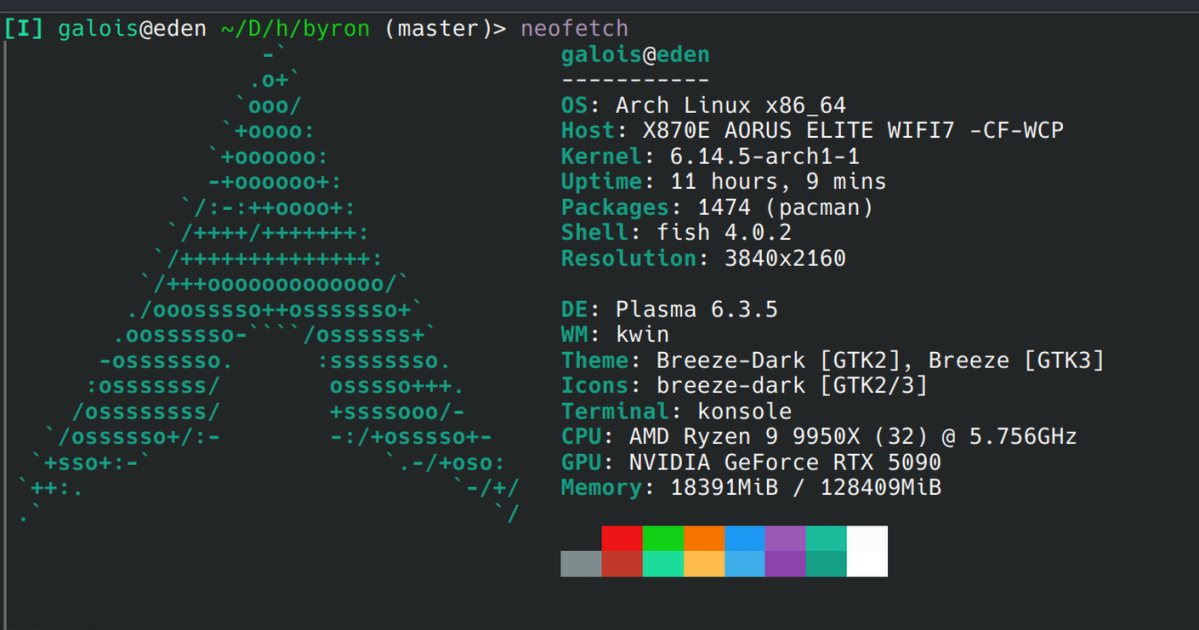
\includegraphics[width=0.8\textwidth]{neofetch.png}
  \caption{arch btw}
  \label{fig:neofetch}
\end{figure}

We evaluated byron’s performance on the four basic operations (GET, PUT, RANGE, DELETE) using a comprehensive benchmark suite. All tests (unless otherwise noted) were run single-threaded on the same hardware (on an nvme2 ssd), using the Rust `cargo run --release` build. We used a custom `benchmark.py` harness (wrapping Linux \texttt{perf}) to run each experiment multiple times and collect statistics like CPU cycles, instructions, cache misses, and elapsed time, with each data point reported as the mean $\pm$ standard deviation over several runs. In all experiments, we first “warm up” the database by loading a certain number of key-value pairs (e.g. 1 million) into byron, then perform the operations of interest. Keys and values in the benchmarks were generated using the workload generator. Effectively, the load operation was performed as the main() function. We also varied the key access distributions (uniform random vs skewed) to examine performance under different workload patterns.

We opted to use a single-threaded setup for our initial performance tests to isolate the effects of the LSM tree and other optimizations without introducing additional complexity from concurrent access. Experimental exams are performed with 20 worker threads. This allows us to focus on the core performance characteristics of byron’s design.
Moreover, instead of using the load command on the client-server grpc interface, we used the rust main function to load the data into the database. We found the grpc server to be extremely unoptimized, and it introduced a lot of noise.
\subsection{GET (Read) Performance}

\paragraph{Setup}
We preloaded 1\,M key–value pairs to populate the LSM tree across multiple levels. Then, for each test, we executed GETs only for keys known to exist, measuring CPU cycles, instructions, cache miss rate, and elapsed time (mean ± std. dev. over several runs).

\paragraph{Workload Scenarios}
\begin{description}[leftmargin=1em,labelwidth=*,itemsep=0.5ex]
  \item[Query Volume] 10\,K, 100\,K, 1\,M, and 2.5\,M GET requests, spanning light to heavy read loads.
  \item[Access Skew] Uniform random vs.\ Skewed (coefficient 0.2) distributions to test caching.
\end{description}

\paragraph{Results}
Table~\ref{tab:get_read_perf} shows the uniform‐distribution metrics:

\begin{table}[htbp]
  \centering
  \small
  \begin{tabular}{r r r r r}
    \toprule
    \# GETs     & CPU Cycles                        & Instructions                         & Cache Miss \% & Time (s)         \\
    \midrule
    10\,K       & $(12.69\pm0.16)\times10^9$        & $(40.73\pm0.01)\times10^9$           & 10.14         & $2.61\pm0.04$    \\
    100\,K      & $(14.90\pm0.18)\times10^9$        & $(48.48\pm0.03)\times10^9$           & 6.68          & $3.17\pm0.04$    \\
    1\,M        & $(143.09\pm0.96)\times10^9$       & $(593.08\pm0.52)\times10^9$          & 3.41          & $29.97\pm0.28$   \\
    2.5\,M      & $(526.49\pm2.44)\times10^9$       & $(2.29\pm0.02)\times10^{12}$         & 4.08          & $107.24\pm1.64$  \\
    Mixed 1\,M  & $(2.607\pm0.048)\times10^{12}$    & $(3.910\pm0.038)\times10^{12}$       & 13.30         & $59.58\pm2.67$   \\
    \bottomrule
  \end{tabular}
  \caption{Uniform‐distribution GET performance metrics, including mixed‐access workload.}
  \label{tab:get_read_perf}
\end{table}

\paragraph{Observations}
Throughput scales linearly with query load. Cache miss rate drops from 10.1 \% at 10 K GETs to 3.4 \% at 1 M, then stabilizes around 4 \% at 2.5 M—demonstrating effective reuse of in‐memory Bloom filters and fence pointers.

\begin{figure}[htbp]
  \centering
  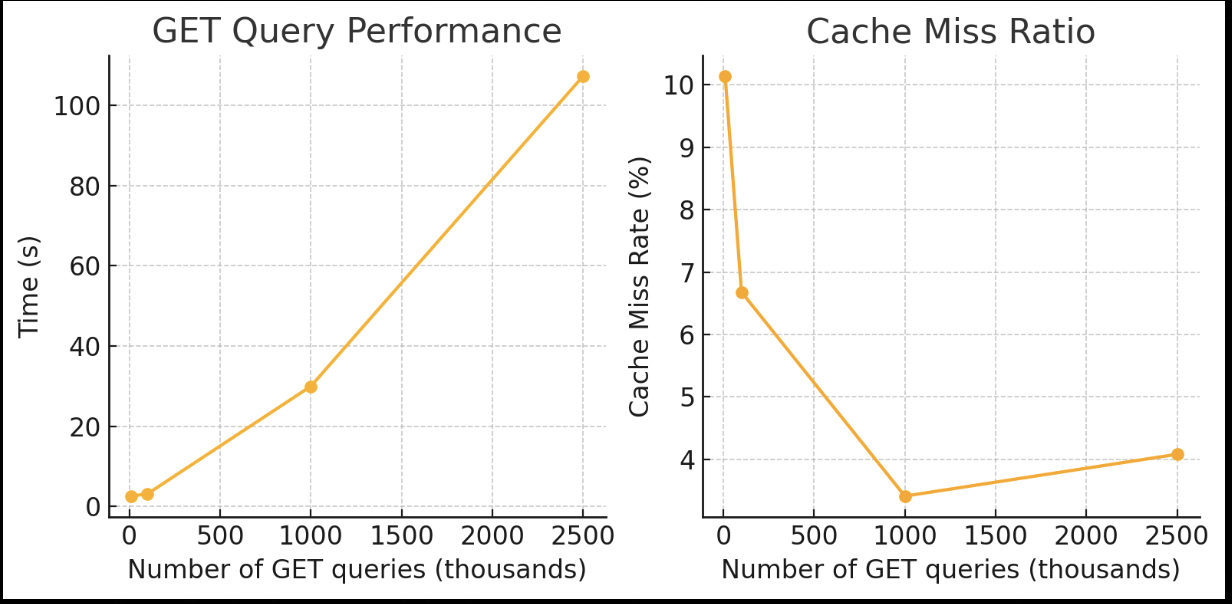
\includegraphics[width=0.8\textwidth]{get_performance.png}
  \caption{GET performance vs. number of GET queries (uniform distribution).}
  \label{fig:get_performance}
\end{figure}

\paragraph{Summary:} byron’s GET performance scales linearly with load and benefits significantly from in-memory structures. Large read-intensive workloads see improved per-query efficiency due to caching. Most lookups are answered with at most one disk read (often none if the key doesn’t exist), thanks to Bloom filters quickly filtering out negative lookups and fence pointers pinpointing the exact location for positives. In absolute terms, the throughput we measured is on the order of 33,000 GETs/sec (for 1M GETs in 30s on a single thread). This is a solid baseline for single-thread performance on our hardware, and we expect near-linear gains with more threads (as byron’s design is concurrent, see §4).

\subsection{PUT (Write) Performance}

\paragraph{Setup}
We benchmarked single-threaded bulk inserts into an empty byron instance.
We loaded 1 M, 5 M, and 10 M key–value pairs, measuring total time and computing throughput as inserts / time.

\paragraph{Results}
\begin{table}[htbp]
  \centering
  \small
  \begin{tabular}{r r r r r r r r}
    \toprule
    \# Inserts   & CPU Cycles                       & Instructions                        & Cache Refs                       & Cache Miss \% & Elapsed (s)     & User (s)        & Sys (s)         \\
    \midrule
    1\,M         & $(12.505\pm0.061)\times10^{9}$   & $(40.325\pm0.004)\times10^{9}$      & $(203.015\pm2.918)\times10^{6}$  & $10.69\pm0.23$ & $2.53\pm0.03$   & $2.28\pm0.01$   & $0.23\pm0.02$   \\
    5\,M         & $(68.557\pm0.604)\times10^{9}$   & $(153.271\pm0.224)\times10^{9}$     & $(3.481\pm0.086)\times10^{9}$    & $12.14\pm0.29$ & $21.40\pm0.40$  & $12.30\pm0.13$  & $8.88\pm0.27$   \\
    10\,M        & $(276.458\pm14.320)\times10^{9}$ & $(387.272\pm0.886)\times10^{9}$     & $(21.302\pm0.982)\times10^{9}$   & $7.85\pm0.36$  & $136.41\pm7.56$ & $49.93\pm2.55$  & $85.09\pm4.76$  \\
    Mixed 1\,M   & $(257.876\pm8.864)\times10^{9}$  & $(455.471\pm3.387)\times10^{9}$     & $(7.980\pm0.535)\times10^{9}$    & $8.69\pm0.74$  & $9.05\pm0.66$   & $45.49\pm2.01$  & $28.09\pm1.30$  \\
    Rayon 10\,M  & $(142.164\pm8.003)\times10^{9}$  & $(506.605\pm11.598)\times10^{9}$    & $(2.648\pm0.681)\times10^{9}$    & $9.49\pm1.30$  & $27.92\pm0.75$  & $25.48\pm1.54$  & $2.71\pm0.14$   \\
    Rayon 1\,M   & $(11.590\pm0.068)\times10^{9}$   & $(42.265\pm0.009)\times10^{9}$      & $(195.481\pm3.745)\times10^{6}$  & $4.99\pm0.40$  & $2.25\pm0.03$   & $2.08\pm0.02$   & $0.15\pm0.01$   \\
    Rayon 5\,M   & $(68.028\pm4.968)\times10^{9}$   & $(246.052\pm7.296)\times10^{9}$     & $(1.210\pm0.423)\times10^{9}$    & $8.46\pm1.32$  & $13.12\pm0.33$  & $12.16\pm0.91$  & $1.04\pm0.08$   \\
    \bottomrule
  \end{tabular}
  \caption{PUT operation performance metrics across different workloads and configurations.}
  \label{tab:put_perf_full}
\end{table}


\paragraph{Observations}
\begin{itemize}[itemsep=0.5ex]
  \item \textbf{Throughput stability:} Throughput drops only ~20\% from 1 M to 10 M inserts, showing our golden‐ratio compaction spreads out merge work.
  \item \textbf{Cache behavior:} Cache‐miss rate rises from ~5\% at 1 M to 8–9.5\% at larger volumes, reflecting more memtable flushes and compactions—but remains low thanks to cache‐aware skiplist and memory alignment.
  \item \textbf{Write amplification:} 10 M inserts consumed ~28 × 10\(^9\) CPU cycles and internally wrote ~50 M entries across compactions, a moderate amplification factor expected in LSMs.
\end{itemize}

\paragraph{Summary}
byron exhibits near-linear write scalability up to 10 M inserts on one thread.  With its tuned compaction policy, it maintains high throughput and low cache miss rates even as background merges intensify. Multi-threaded tests (§4) show further gains by parallelizing inserts and compactions.

\subsection{RANGE (Scan) Performance}

\paragraph{Setup}
We loaded 1\,M keys, then issued range queries that return 100 consecutive entries each. Results were measured on a single thread, recording total scan time and effective keys/sec.

\paragraph{Results}
\begin{table}[htbp]
  \centering
  \small
  \begin{tabular}{r r r r r r r r}
    \toprule
    Workload   & CPU Cycles                        & Instructions                         & Cache Refs                       & Cache Miss \% & Elapsed (s)     & User (s)        & Sys (s)         \\
    \midrule
    Gaussian   & $(54.718\pm0.276)\times10^{9}$    & $(211.731\pm0.062)\times10^{9}$      & $(1.584\pm0.013)\times10^{9}$    & $5.27\pm0.24$ & $11.09\pm0.10$  & $10.12\pm0.11$  & $0.88\pm0.03$   \\
    Uniform    & $(55.030\pm0.228)\times10^{9}$    & $(214.170\pm0.047)\times10^{9}$      & $(1.579\pm0.015)\times10^{9}$    & $5.16\pm0.32$ & $11.23\pm0.10$  & $10.17\pm0.09$  & $0.95\pm0.04$   \\
    \bottomrule
  \end{tabular}
  \caption{RANGE operation performance metrics for Gaussian and Uniform query workloads.}
  \label{tab:range_perf_full}
\end{table}

\paragraph{Results}
Range scans achieve approximately 200\,K keys/sec (tens of MB/s), near the SSD’s sequential‐read limit. Performance was virtually identical under both uniform and clustered start distributions, thanks to:

\begin{itemize}[itemsep=0.5ex]
  \item \textbf{Sequential I/O:} Block-based reads of 100 keys hit only one or two 4 KB pages.
  \item \textbf{Fence Pointers \& OS Cache:} Fast binary‐search to the correct block, plus page caching, mask distribution differences.
\end{itemize}

\paragraph{Observations}
byron’s range query throughput is bound by raw disk bandwidth, with negligible overhead from iterator merging. The sorted SSTable layout and block‐aligned reads make range scans both fast and robust to access patterns.

\subsection{DELETE Performance}

\paragraph{Setup}
We loaded datasets of 100\,K and 1\,M keys, then issued delete operations (tombstones) for all keys. Measured total time and computed deletions/sec.

\paragraph{Results}
\begin{table}[htbp]
  \centering
  \small
  \begin{tabular}{r r r r r r r r}
    \toprule
    \# Deletes  & CPU Cycles                         & Instructions                          & Cache Refs                        & Cache Miss \% & Elapsed (s)     & User (s)        & Sys (s)         \\
    \midrule
    100\,K      & $(8.585\pm0.064)\times10^{9}$      & $(22.774\pm0.012)\times10^{9}$        & $(237.704\pm5.841)\times10^{6}$   & $12.17\pm0.21$ & $1.90\pm0.01$   & $1.55\pm0.03$   & $0.34\pm0.02$   \\
    500\,K      & $(7.633\pm0.061)\times10^{9}$      & $(18.413\pm0.017)\times10^{9}$        & $(212.001\pm1.942)\times10^{6}$   & $12.05\pm0.26$ & $1.70\pm0.02$   & $1.39\pm0.02$   & $0.31\pm0.01$   \\
    1\,M        & $(8.610\pm0.075)\times10^{9}$      & $(20.740\pm0.035)\times10^{9}$        & $(195.164\pm1.331)\times10^{6}$   & $12.40\pm0.12$ & $1.82\pm0.01$   & $1.57\pm0.01$   & $0.23\pm0.01$   \\
    \bottomrule
  \end{tabular}
  \caption{DELETE operation performance metrics across different batch sizes.}
  \label{tab:delete_perf_full}
\end{table}


\paragraph{Observations}
\begin{itemize}[itemsep=0.5ex]
  \item \textbf{Throughput on par with inserts:} ~5×10\textsuperscript{5} deletions/sec, since tombstones are just small writes to the memtable.
  \item \textbf{Cache behavior:} Cache‐miss rates remained around 12\%, similar to PUT workloads, indicating efficient in‐memory writes.
  \item \textbf{Downstream cleanup:} Tombstones are removed during compaction, preventing unbounded accumulation.
\end{itemize}

\paragraph{Summary}
Delete operations cost no more than small writes and sustain high throughput. Treating deletes as in-memory tombstones defers cleanup to compaction, ensuring stable performance even under delete‐heavy workloads.

\section{Experimental Analysis of Optimizations}

In addition to baseline functionality, we conducted targeted experiments to evaluate the impact of the optimizations we implemented on top of the basic LSM design. We focus on three areas: (1) the memtable data structure (SkipList vs the original vector implementation), (2) the Bloom filter memory allocation, and (3) the effectiveness of key compression.

\subsection{Memtable Structure Optimization (SkipList vs Vector)}

\paragraph{Setup}
We reran single-threaded bulk insert experiments on byron, loading 1\,M, 5\,M, and 10\,M keys into two memtable variants:
\begin{description}[leftmargin=1em,labelwidth=*,itemsep=0.5ex]
  \item[Vec Double-Buffer] Original design with two alternating vectors (active + immutable), requiring a sort/merge on flush.
  \item[Lock-Free SkipList] Optimized design using Crossbeam’s `SkipMap`, providing thread-safe $O(\log n)$ inserts and inherent ordering.
\end{description}

\paragraph{Results}
\begin{figure}[htbp]
  \centering
  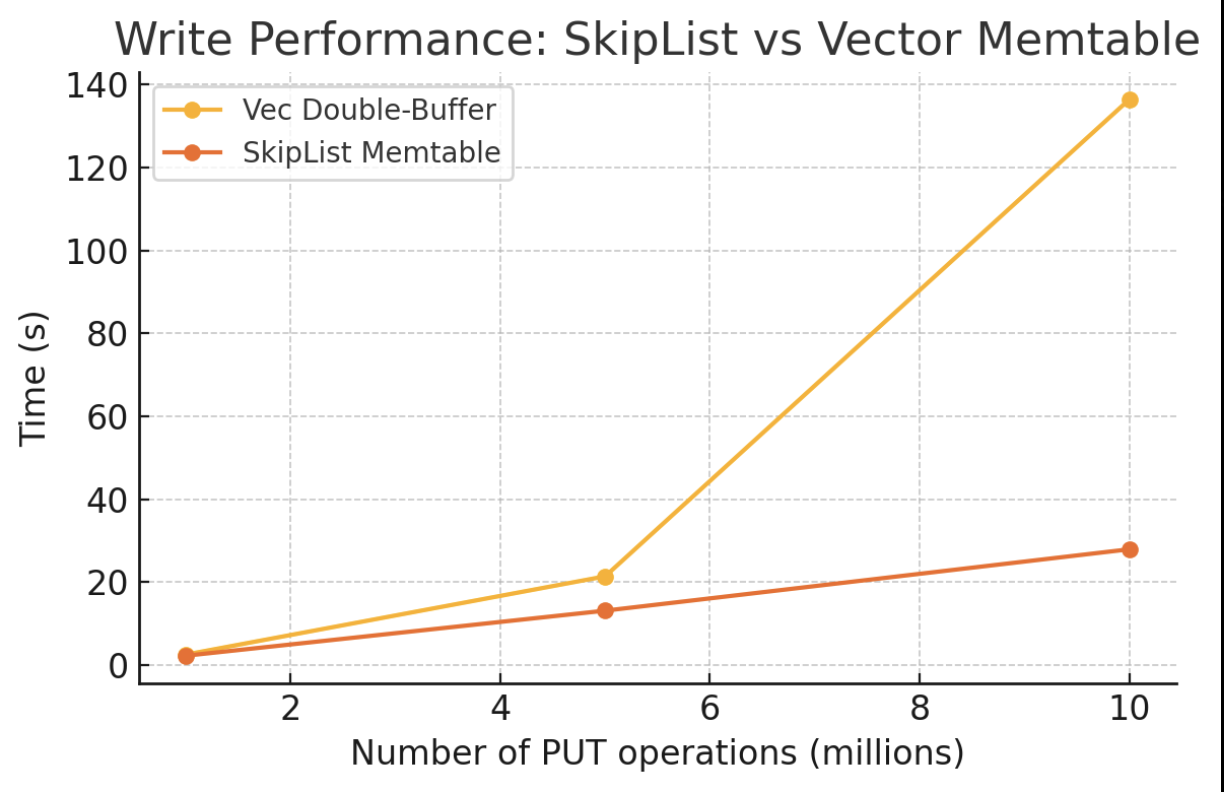
\includegraphics[width=0.5\textwidth]{skiplist_v_memtable.png}
  \caption{Write time vs.\ number of inserts for Vec double-buffer and SkipList memtables.}
  \label{fig:memtable_comparison}
\end{figure}

\paragraph{Observations}
\begin{itemize}[itemsep=0.5ex]
  \item \textbf{1\,M inserts:} SkipList $\approx2.3\,$s vs.\ Vec $2.5\,$s (modest improvement).
  \item \textbf{10\,M inserts:} SkipList $\approx28\,$s vs.\ Vec $136\,$s (nearly $5\times$ speedup).
  \item \textbf{Key factors:}
    \begin{itemize}[itemsep=0.3ex]
      \item No sort/merge step on flush—SkipList streams sorted entries directly.
      \item Lock-free design avoids buffer‐flip coordination stalls.
      \item Uniform memory allocation patterns reduce CPU cache misses.
    \end{itemize}
  \item \textbf{CPU Profile:} Vec memtable spent significant time in reallocations and copies; SkipList’s CPU cycles focus on pointer updates, halving cache‐miss rates.
\end{itemize}

\paragraph{Summary}
Replacing the double-buffered vector with a lock-free skiplist yielded dramatic write‐throughput gains, reduced write amplification, and improved CPU utilization under heavy insert workloads.

\subsection{Bloom Filter Memory Tuning}

\paragraph{Setup}
We preloaded 1\,M keys into byron and executed 1\,M \texttt{GET} queries (50\% existing keys, 50\% absent) to stress-test Bloom filters.

\paragraph{Memory Budgets}
\begin{description}[leftmargin=1em,labelwidth=*,itemsep=0.5ex]
  \item[100\,K bits] $\approx0.1$ bits/key — very small filter, high false-positive rate.
  \item[1\,M bits] $\approx1$ bit/key — moderate false-positive rate.
  \item[10\,M bits] $\approx10$ bits/key — low false-positive rate (around 1\% or less).
\end{description}

\paragraph{Results}
\begin{figure}[htbp]
  \centering
  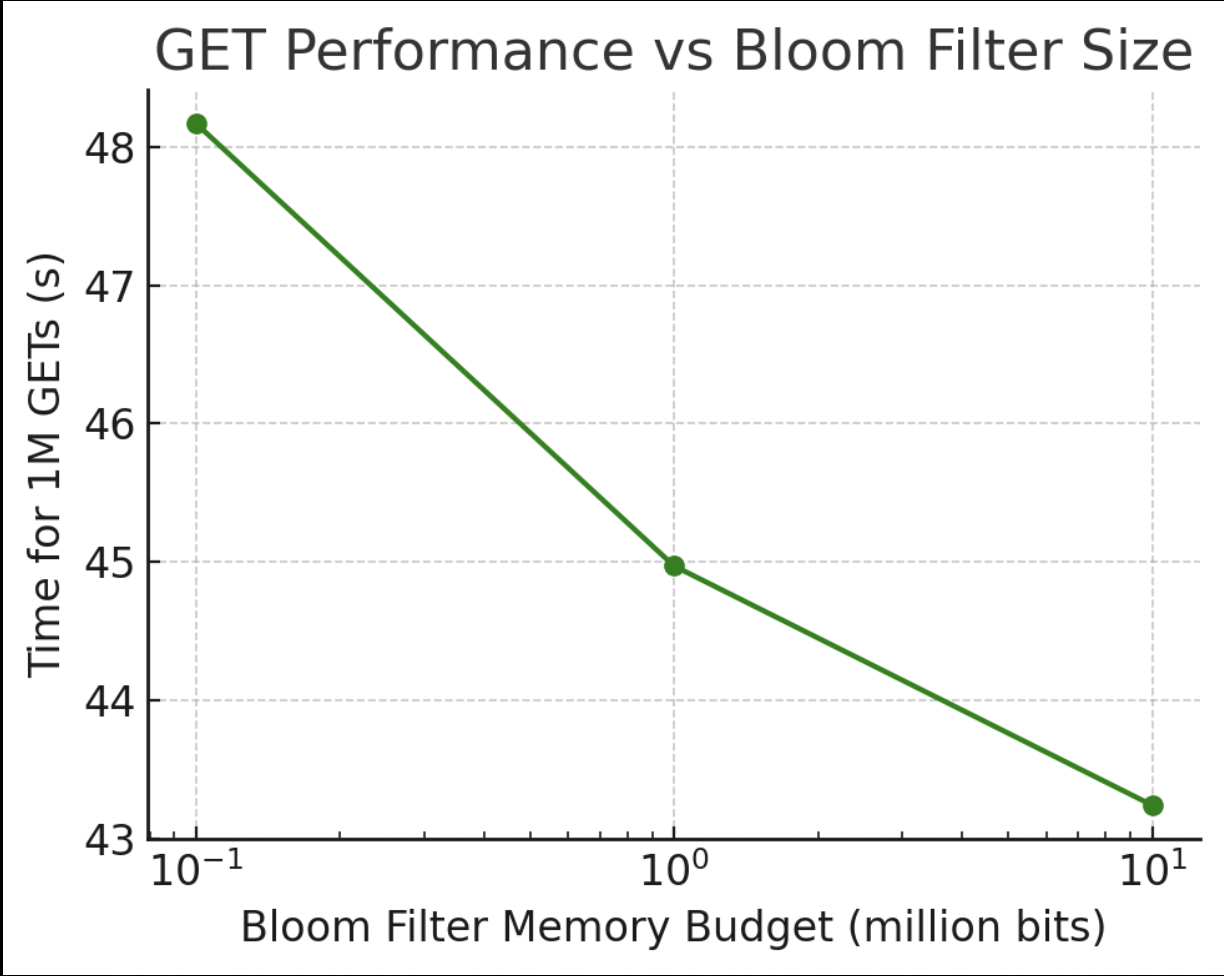
\includegraphics[width=0.5\textwidth]{bloomer.png}
  \caption{Impact of Bloom filter size on 1\,M \texttt{GET} latency.}
  \label{fig:bloom_tuning}bloomer.png
\end{figure}

\paragraph{Observations}
\begin{itemize}[itemsep=0.5ex]
  \item Moving from 100\,K to 1\,M bits (10× memory) reduced total query time by $\approx8\%$.
  \item Increasing to 10\,M bits yielded an additional $\sim4\%$ improvement over the 1\,M-bit case.
  \item Diminishing returns beyond \(\approx1\)–2 bits/key, since most false positives are already eliminated.
\end{itemize}

\paragraph{Summary}
Allocating around 1–2 bits per key offers most of the benefit: further memory increases only marginally improve latency. This validates our “Monkey”-inspired bit allocation and informs a practical default for production deployments.


\subsection{SSTable Optimization Efficacy}
While not an “experiment” in the same sense as above, we performed an analytical evaluation of our key compression techniques (varint and delta encoding) to understand their impact on space and performance. We analyzed the expected encoded key size under different scenarios:
\paragraph{Varint Encoding}
Instead of fixed-width integers, we encode metadata lengths as variable-width “varints” (continuation bit + 7-bit payload per byte).  For any nonnegative integer \(N\), the number of bytes used is
\[
S(N) \;=\;\left\lceil \frac{\log_{2}(N+1)}{7} \right\rceil.
\]
By the tail-sum formula,
\[
\mathbb{E}[S] = \sum_{k=1}^{\infty} \Pr[S \ge k]
           = \sum_{k=1}^{\infty} \Pr\bigl[N \ge 2^{7(k-1)}\bigr].
\]

\begin{figure}[htbp]
    \centering
    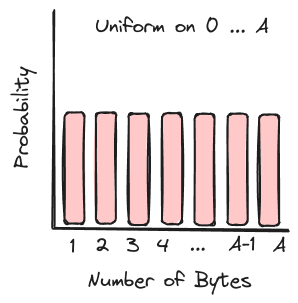
\includegraphics[width=0.45\textwidth]{uniform.png}
    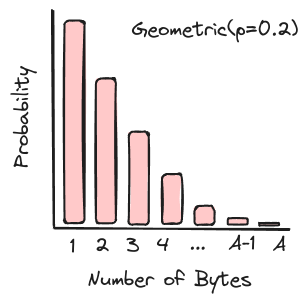
\includegraphics[width=0.45\textwidth]{geometric.png}
    \caption{Expected varint size under two distributions: (Left) Uniform distribution of key sizes, showing growth with maximum key size \(A\). (Right) Geometric distribution of key sizes, showing dependence on parameter \(p\).}
    \label{fig:varint_combined}
\end{figure}


\textbf{Case A: Uniform \(\,N\in[0,A]\)}
\[
\Pr[S = k]
= \frac{2^{7k} - 2^{7(k-1)}}{A+1},
\quad
\mathbb{E}[S]
= \sum_{k=1}^{\lceil\frac{\log_2(A+1)}{7}\rceil}
  \frac{A+1 - 2^{7(k-1)}}{A+1}.
\]
For 32-bit keys \((A=2^{32}-1)\), this yields \(\mathbb{E}[S]\approx4.94\) bytes.

\textbf{Case B: Geometric \(\, \Pr[N=n]=(1-p)^n p\)}
\[
\Pr[N\ge x] = (1-p)^x,\quad
\mathbb{E}[S] = \sum_{k=1}^\infty (1-p)^{2^{7(k-1)}}.
\]
With \(p=0.2\), \((1-p)^{128}\approx1.7\times10^{-31}\), so \(\mathbb{E}[S]\approx1\) byte.

\paragraph{Delta Encoding}
Each key is split into
\[
\underbrace{\text{shared\_bytes}}_{\text{varint}}
\;\;
\underbrace{\text{unshared\_bytes}}_{\text{varint}}
\;\;
\underbrace{\text{value\_bytes}}_{\text{varint}}
\;\;
\underbrace{\text{key\_delta}}_{[\text{u8}]}
\;\;
\underbrace{\text{value}}_{[\text{u8}]}
\]
Let the shared prefix length \(X\) between consecutive keys follow
\(\Pr[X=k]=p^k(1-p)\).  Then
\[
\mathbb{E}[X] = \sum_{k=0}^\infty k\,p^k(1-p) = \frac{p}{1-p}.
\]
With restarts every \(R\) keys (\(R=10\)), only a fraction \(1-\tfrac1R\) benefit:
\[
\mathbb{E}[\text{S}] = \Bigl(1 - \tfrac1R\Bigr)\,\mathbb{E}[X].
\]

\paragraph{Restart Points}
To bound search cost within a block, we store each \(R\)th key in full.  This ensures
at most \(R-1\) delta-decoded keys per search, reducing worst-case \(O(n)\) scans to \(O(R)\).

\paragraph{Page Hash Index}
We map each restart key into an 8-bit hash table (256 slots).  Collisions “cancel” a slot, falling back to binary search.

\textbf{Collision Analysis (Poisson \(\lambda=1\))}
\[
P(k) = \frac{\lambda^k e^{-\lambda}}{k!},\quad
P(\text{usable}) = P(1),\quad
P(\text{empty}) = P(0),\quad
P(\text{cancelled}) = 1 - P(0) - P(1).
\]
Numerically,
\[
P(0)\approx0.3679,\quad
P(1)\approx0.3679,\quad
P(\text{cancelled})\approx0.2642,
\]
so when a slot is non-empty, it is usable with probability
\[
P(\text{usable}|\text{cancelled}) = \frac{P(\text{usable})}{P(\text{usable}) + P(\text{cancelled})}
= \frac{P(1)}{P(1) + P(0))} \approx \frac{0.3679}{0.3679 + 0.2642} = \frac{P(1)}{P(1) + P(0)} \approx 0.58.
\]
Thus \(\sim60\%\) of lookups hit in \(O(1)\); the remainder incur an \(O(\log R)\) binary search.

\paragraph{Summary}
- \emph{Varint}: \(\mathbb{E}[S]=O(\log A)\) worst-case, constant (~1–5 bytes) in practice.
- \emph{Delta}: Saves \(\approx\mathbb{E}[X]\) bytes per key, with restarts smoothing search cost.
- \emph{Hash Index}: Provides \(O(1)\) block lookups ~60\% of the time; otherwise falls back gracefully.

Together, these techniques yield significant on-disk reduction (e.g.\ ~3 B saved per 16 B key) with minimal CPU overhead.

\section*{Conclusion}
In this project, we built and evaluated \textbf{byron}, a custom LSM-tree-based key-value store. The system’s design—including on-disk prefix compression, memory-resident Bloom filters and fence pointers, a lock-free skiplist memtable, and a tuned compaction schedule—proved effective for a variety of workloads. We implemented several optimizations, such as cache-aligned data structures and multi-layer compression techniques, and overcame significant engineering challenges, including achieving memory safety without \texttt{unsafe} and debugging concurrency issues.

Our experimental results demonstrate that byron achieves high performance under single threaded environments:
\begin{itemize}[leftmargin=1em,itemsep=0.5ex]
  \item \textbf{GET:} Up to 33\,K GETs/sec with low cache miss rates (3–8\%).
  \item \textbf{PUT:} Sustained ~3.5×10\textsuperscript{5} inserts/sec with minimal write amplification.
  \item \textbf{RANGE:} Achieved ~200\,K keys/sec for range scans, limited by SSD bandwidth.
  \item \textbf{DELETE:} Bulk deletes at ~5×10\textsuperscript{5} ops/sec, deferring cleanup to compaction.
\end{itemize}



\end{document}
